% Created 2013-06-13 czw 18:15
\documentclass[presentation, 10pt]{beamer}
\usepackage[utf8]{inputenc}
\usepackage[utf8]{inputenc}
\usepackage[T1]{fontenc}
\usepackage{fixltx2e}
\usepackage{graphicx}
\usepackage{longtable}
\usepackage{float}
\usepackage{wrapfig}
\usepackage{soul}
\usepackage{textcomp}
\usepackage{marvosym}
\usepackage{wasysym}
\usepackage{latexsym}
\usepackage{amssymb}
\usepackage{hyperref}
\tolerance=1000
\usepackage{minted}
\usepackage{amsfonts}
\usepackage{amsmath}
\usepackage[polish]{babel}
\usepackage{polski}
\usepackage[export]{adjustbox}
\usepackage{tikz}
\usetikzlibrary{mindmap, trees, arrows, decorations.markings}
\usetheme{Madrid}
\usefonttheme{structurebold}
\usecolortheme{default}
\beamertemplateballitem
\setbeamersize{text margin left=5mm}
\setbeamercovered{transparent}
\setbeamertemplate{navigation symbols}{}
\institute[IS]{Informatyka Stosowana}
\author[M. Lenart, M. Rzeszutek, D. Świętek]{Michał Lenart, Mateusz Rzeszutek, Dariusz Świętek}
\AtBeginSection[]{\frame<handout:0>{\frametitle[allowframebreaks]{Plan prezentacji}\tableofcontents[current]}}
\providecommand{\alert}[1]{\textbf{#1}}

\title{Domofon}
%\author{mateusz}
\date{\today}
\hypersetup{
  pdfkeywords={},
  pdfsubject={},
  pdfcreator={Emacs Org-mode version 7.9.3f}}

\begin{document}

\maketitle






\section{Wstęp}
\label{sec-1}
\begin{frame}
\frametitle{Opis zadania}
\label{sec-1-1}

Celem projektu jest zbudowanie bezprzewodowego domofonu z wykorzystaniem wbudowanej
platformy komputerowej SoC (np. Zedboard lub Raspberry Pi) opartej na systemie Linux. Karta
wyposażona jest w port wejścia/wyjścia umożliwiający pobieranie oraz wysyłanie informacji
poprzez linie cyfrowe. System będzie się składał z dwóch elementów:
\begin{itemize}
\item ``panel zewnętrznego'' składający się z platformy SoC wyposażony w moduł komunikacji
  poprzez sieć bezprzewodową, zestaw przycisków i kontrolek LED,
\item ``panel wewnętrzny'' składający się z komputera (lub np. kolejnej platformy SoC) z
  zestawem przycisków oraz system sygnalizacji dźwiękowej.
\end{itemize}
\end{frame}
\section{Koncept}
\label{sec-2}
\begin{frame}
\frametitle{Koncept}
\label{sec-2-1}

  \begin{tikzpicture}[scale=1.4]
    \tikzstyle{elem} = [ultra thick, rounded corners, rectangle, draw=blue!80, scale = 1.5, inner sep = 0.5cm]
    \tikzstyle{sip} = [ultra thick, rounded corners, rectangle, draw=orange!80, scale = 1.5, inner sep = 0.5cm]
  
    \node[elem] (rpi) at (6, 0) {Domofon};
    \node[elem] (pc) at (0, 0) {Klient};
    \node[sip] (sip) at (3, 3) {Serwer SIP};
  
    \foreach \from/\to in {rpi/pc, rpi/sip, pc/sip}
    \draw [<->, very thick, >=triangle 60] (\from) -- (\to);
  \end{tikzpicture}
\end{frame}
\section{Implementacja}
\label{sec-3}
\begin{frame}
\frametitle{Użyty sprzęt}
\label{sec-3-1}

\begin{itemize}
\item Raspberry Pi, wersja B
\item no-name mikrofon
\item no-name karta dźwiękowa USB
\item głośniki
\item wyświetlacz LCD 16 \texttimes{} 2
\item 3 przyciski
\item kabelki
\end{itemize}
\end{frame}
\begin{frame}
\frametitle{Użyte technologie}
\label{sec-3-2}

Serwer:
\begin{itemize}
\item Python
\item GPIO
\item prosty serwer http (cherrypy)
\item linphonecsh
\end{itemize}

Klient:
\begin{itemize}
\item Python
\item kivy
\item linphone
\end{itemize}
\end{frame}
\begin{frame}
\frametitle{Serwer (domofon)}
\label{sec-3-3}

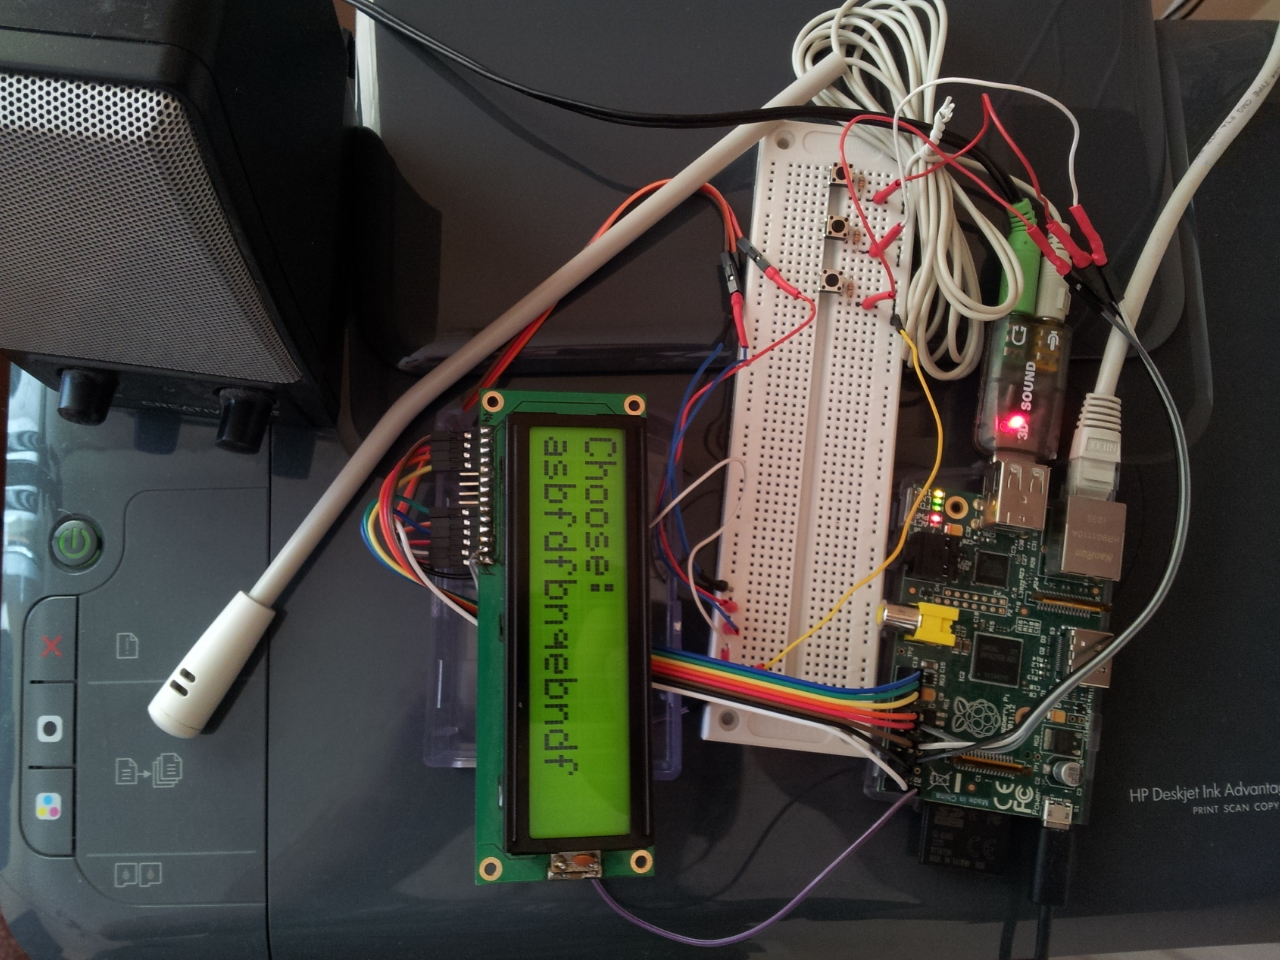
\includegraphics[width=.9\linewidth]{rpi1.jpg}
\end{frame}
\begin{frame}
\frametitle{Klient (aplikacja)}
\label{sec-3-4}

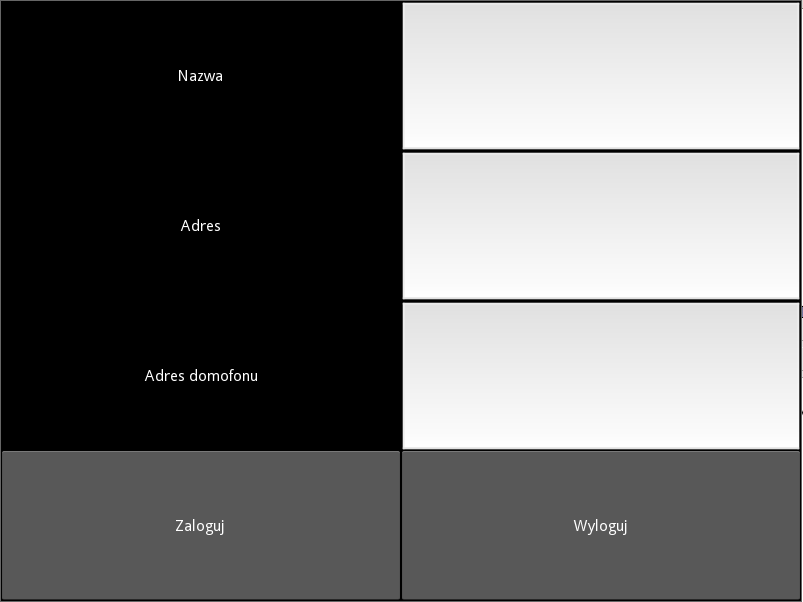
\includegraphics[width=.9\linewidth]{client.png}
\end{frame}
\begin{frame}
\frametitle{Future work}
\label{sec-3-5}

\begin{itemize}
\item \textbf{Strumieniowanie} \\
Pozbycie się linphone'a, i zaimplementowanie strumieniowania audio (np. za pomocą biblioteki gstreamer).
\item \textbf{Interfejs WiFi} \\
Zakup interfejsu WiFi.
\item \textbf{Opakowanie} \\
Zrobienie obudowy/pudełka na układ (teraz poszczególne części leżą ``gołe'', trzymając się tylko na kabelkach).
\end{itemize}
\end{frame}
%% Koniec
\label{sec-4}
\begin{frame}

  \begin{center}
    \large{
      Pytania?
      \\ 
      \vfill
      Dziękujemy za uwagę.
    }
    \vspace{1em}
  \end{center}
\end{frame}

\end{document}
